\begin{figure*}
    \centering
    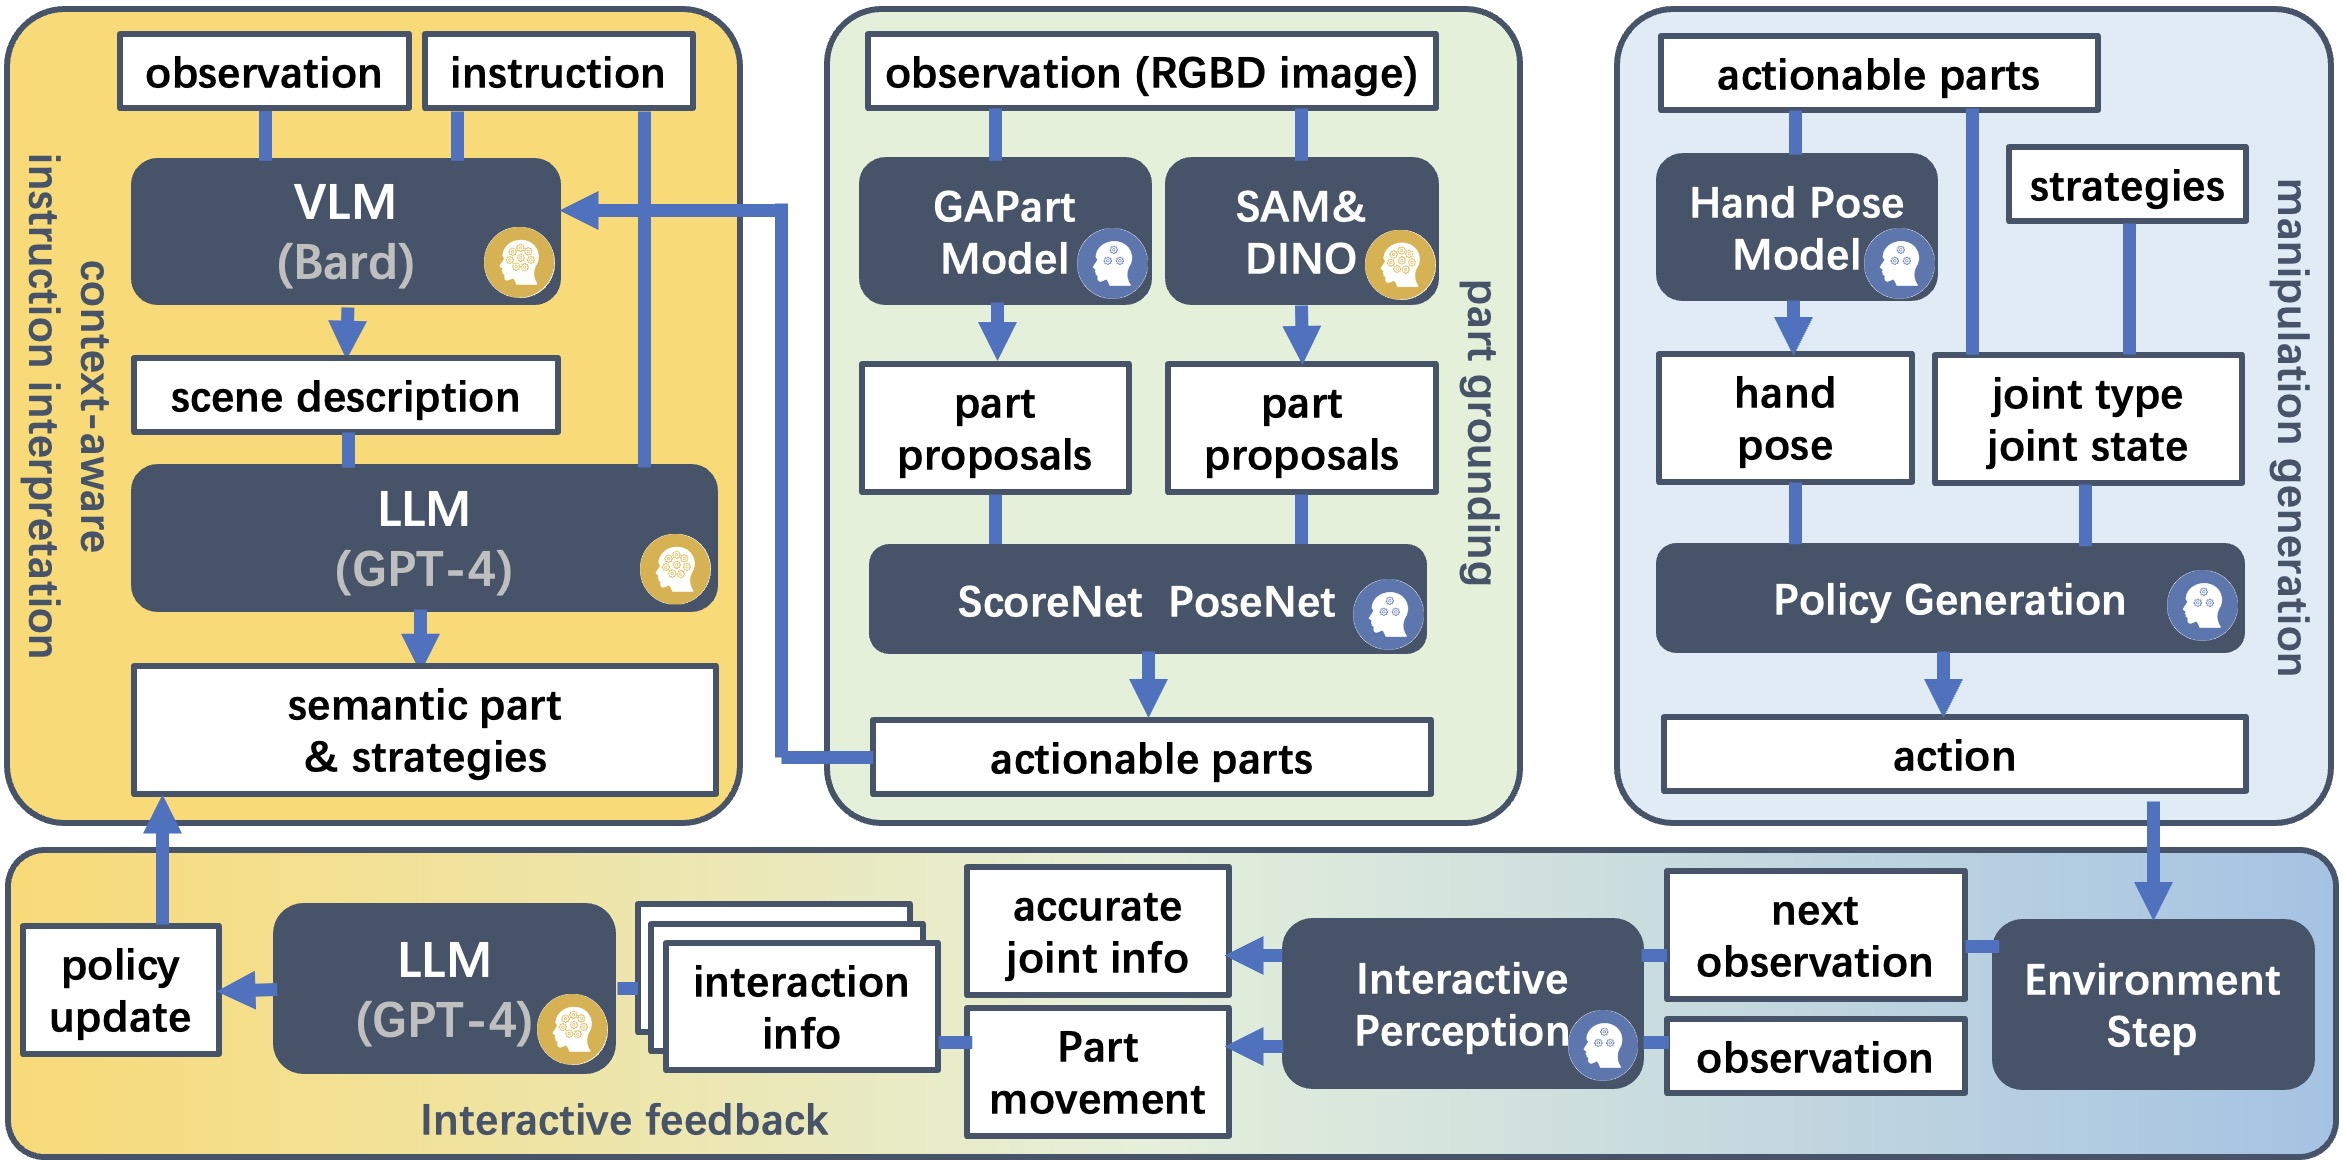
\includegraphics[width=.8\linewidth]{figures/pipeline_new.jpg}
    \caption{
    \textbf{Method Overview.} Our pipeline takes the human manipulation instruction and the first scene observation (RGBD image) as input. With a \textbf{context-aware instruction interpretation module}, we generate target semantic parts and corresponding strategies. Then a \textbf{part grounding module} is used to estimate part state and actionable part information. The \textbf{manipulation generation module} then generates the physics-plausible actions to finish the task. During the interaction, compared with nearby observations of two frames, the \textbf{interactive feedback module} updates the joint state and part movement as interaction information, which is further fed into the planning LLM module to update the interaction policy.
    \CD{Hand pose model -> gripper pose model, as we're not working with dexterous hands?}
    \CD{We still have some space here, maybe we can add some images of inputs/outputs}
    }
    \label{fig:pipe}
\end{figure*}